\documentclass[../main.tex]{subfiles}

\usepackage{nopageno} %Seitenzahlen auf richtiger Seite 

\usepackage[left=2cm, right=2cm, top=2cm, includehead, includefoot, headheight=17pt]{geometry}

\usepackage[utf8x]{inputenc}
\usepackage[english]{babel}
\usepackage{amsmath,amssymb,amsthm}
\usepackage{framed}
\usepackage{wasysym}
\usepackage[T1]{fontenc} %Silbentrennung 
\usepackage{color} %Farbe
\usepackage{graphicx}
\usepackage{float}%Grafik am gleichen Ort plazieren
%pdf. png. einfach eingliedern
\usepackage{subfigure} %Grafiken nebeneinander
\usepackage{pdfpages}
\usepackage{ulem} 	%\uuline{urgent}    % doppelt unterstreichen
%\uwave{boat}      % unterschlängeln
%\sout{wrong}       % durchstreichen
%\xout{removed}     % ausstreichen mit //////.

\usepackage{tikz}
\usetikzlibrary{trees}
\usetikzlibrary{plotmarks}
\usetikzlibrary{angles,quotes,babel}
\usetikzlibrary{shadings}
\usetikzlibrary{patterns}
\usetikzlibrary{matrix}
\usetikzlibrary{arrows}
\usetikzlibrary{calc}

\usepackage{pgfplots}
\usepackage{pgf-pie}
\pgfplotsset{compat=1.10}
\usepgfplotslibrary{statistics}
\usepgfplotslibrary{fillbetween}

\usepackage{tkz-euclide}
\usepackage{enumerate}
\usepackage{stmaryrd}
\usepackage{tabularx}
\usepackage{wrapfig}
\usepackage{epsdice}
\usepackage{multirow}
\usepackage{rotating}
\usepackage{pdflscape}
\usepackage{fancyhdr}

\pagestyle{fancy} %eigener Seitenstil
\fancyhf{} %alle Kopf- und Fußzeilenfelder bereinigen
\fancyhead[L]{} %Kopfzeile links
\fancyhead[C]{} %zentrierte Kopfzeile
\fancyhead[R]{} %Kopfzeile rechts
\renewcommand{\headrulewidth}{0.4pt} %obere Trennlinie
\fancyfoot[C]{\thepage} %Seitennummer
\renewcommand{\footrulewidth}{0.4pt} %untere Trennlinie

% Number spaces 
\newcommand{\CC}{\ensuremath{\mathbb{C}}}
\newcommand{\RR}{\ensuremath{\mathbb{R}}}
\newcommand{\QQ}{\ensuremath{\mathbb{Q}}}
\newcommand{\ZZ}{\ensuremath{\mathbb{Z}}}
\newcommand{\NN}{\ensuremath{\mathbb{N}}}
\newcommand{\LL}{\ensuremath{\mathbb{L}}}
\newcommand{\DD}{\ensuremath{\mathbb{D}}}
\newcommand{\WW}{\ensuremath{\mathbb{W}}}

%draw chemestry molecules 
\usepackage{chemfig} % https://mirror.ox.ac.uk/sites/ctan.org/macros/generic/chemfig/

\newcommand\vv[1]{%
	\begin{tikzpicture}[baseline=(arg.base)]
		\node[inner xsep=0pt] (arg) {$#1$};
		\draw[line cap=round,line width=0.45,->,shorten >= 0.2pt, shorten <= 0.7pt] (arg.north west) -- (arg.north east);
	\end{tikzpicture}%
} %command will render \vv{x} with an arrow aboth 

\renewcommand{\labelenumi}{\roman{enumi})}

\DeclareMathOperator{\ggT}{ggT}
\DeclareMathOperator{\sign}{sign}

%sections
\theoremstyle{plain}
\newtheorem{Thm}{Theorem}[section]
\newtheorem{Def}[Thm]{Definition}
\newtheorem{Prop}[Thm]{Proposition}

\theoremstyle{definition}
\newtheorem{lemma}[Thm]{Lemma}
\newtheorem{corollary}[Thm]{Corollary}
\newtheorem{claim}[Thm]{Claim}
\newtheorem{Proof}[Thm]{Proof}
\newtheorem{Ex}[Thm]{Example}

\newtheorem{Exercise}{ex}[section] %follow proper enum
\newtheorem{ex}[Exercise]{Exercise}
\newtheorem{Solution}{sol}[section]
\newtheorem{sol}[Solution]{Solution}

\theoremstyle{remark}
\newtheorem{remark}[Thm]{Remark} % follows thm enum

\newtheorem{comment}{Comment}[section] %follow comment enum
\newtheorem{notation}[comment]{Notation}
\newtheorem{reasoning}[comment]{Reasoning}
\newtheorem{Intpr}[comment]{Interpretation}

%some premmade with title (uterwise use \textbf{Title} ...)
\newenvironment{ThmWithTitle}[1]{%
	\begin{Thm}[\textbf{#1}]}{\end{Thm}}
\newenvironment{PropWithTitle}[1]{%
	\begin{Prop}[\textbf{#1}]}{\end{Prop}}
\newenvironment{ExWithTitle}[1]{%
	\begin{Ex}[\textbf{#1}]}{\end{Ex}}
\newenvironment{DefWithTitle}[1]{%
	\begin{Def}[\textbf{#1}]}{\end{Def}}
\newenvironment{RemarkWithTitel}[1]{%
	\begin{remark}[\textbf{#1}]}{\end{remark}}

%format of paragraph 
\renewcommand\paragraph{\@startsection{paragraph}{4}{\z@}%
	{-2.5ex\@plus -1ex \@minus -.25ex}%
	{1.25ex \@plus .25ex}%
	{\normalfont\normalsize\bfseries}}
\makeatother
\setcounter{secnumdepth}{4} % how many sectioning levels to assign numbers to
\setcounter{tocdepth}{4}    % how many sectioning levels to show in ToC

\newcounter{row} 
\renewcommand\therow{\alph{row}} %hier a,b,c etc. def und mit therow abrufbar

\newenvironment{aufz}
{\setcounter{row}{0}%
	\par\noindent\tabularx{\linewidth}[t]
	{\cdot{20}{>{\stepcounter{row}\makebox[1.5em][l]{\therow)\hfill}}X}} %bis max 20 Elemente nebeinander
}
{\endtabularx}


%biblio
\usepackage[]{biblatex}
\addbibresource{referenzenma.bib} 

%glossary
\usepackage{glossaries}
\usepackage{import}


\usepackage{rotating} % Include this package in the preamble

\newglossaryentry{electrochemicalgradient}{
	name={electrochemical gradient},
	description={A gradient formed by the combined effect of an ion's concentration gradient and the electrical potential across a membrane. It determines the direction and force with which ions move across biological membranes},
	sort=electrochemicalgradient
}
\newglossaryentry{uniporter}{
	name=Uniporter,
	description={Transporter that facilitates the movement of a single type of molecule or ion across the membrane down its concentration gradient (passive transport), without coupling to the movement of any other substance}
}

\newglossaryentry{symporter}{
	name=Symporter,
	description={A cotransporter that moves two (or more) different substances across a membrane in the same direction. One substance typically moves down its electrochemical gradient, providing the energy to transport the other substance against its gradient}
}

\newglossaryentry{antiporter}{
	name=Antiporter,
	description={A cotransporter that exchanges two (or more) substances across a membrane in opposite directions. Movement of one substance down its electrochemical gradient powers the transport of another substance against its gradient}
}

\newglossaryentry{primaryactivetransport}{
	name=Primary active transport,
	description={A form of active transport that directly uses energy, usually from the hydrolysis of ATP, to move molecules or ions against their electrochemical gradient across a membrane. Example: the Na\textsuperscript{+}/K\textsuperscript{+}-ATPase pump}
}

\newglossaryentry{secondaryactivetransport}{
	name=Secondary active transport,
	description={A type of active transport that does not use ATP directly. Instead, it relies on the electrochemical gradient established by primary active transport to drive the movement of other substances against their gradients. Can be in the form of symport or antiport}
}

\newglossaryentry{SGLT}{
	name=SGLT family,
	description={Sodium-Glucose Linked Transporters are secondary active transporters that couple the uptake of glucose with the inward movement of Na\textsuperscript{+} ions, enabling glucose absorption against its concentration gradient. Prominent in intestinal and renal epithelial cells}
}

\newglossaryentry{osmolarity}{
	name=Osmolarity,
	description={The total concentration of solute particles in a solution, measured in osmoles per liter (Osm/L). It governs water movement across membranes and is regulated in cells in part by ion pumps like the Na\textsuperscript{+}/K\textsuperscript{+} pump}
}

\newglossaryentry{isotonic}{
	name=Isotonic,
	description={Describes a solution that has the same osmolarity as the inside of a cell, resulting in no net movement of water across the cell membrane}
}

\newglossaryentry{hypertonic}{
	name=Hypertonic,
	description={Describes a solution with higher osmolarity than the cell interior, causing water to leave the cell and leading to cell shrinkage}
}

\newglossaryentry{hypotonic}{
	name=Hypotonic,
	description={Describes a solution with lower osmolarity than the cell interior, causing water to enter the cell and potentially leading to cell swelling or lysis}
}

\newglossaryentry{sarcoplasmicreticulum}{
	name={sarcoplasmic reticulum (SR)}, 
	description={The SR is a specialized type of endoplasmic reticulum that forms a network of tubular sacs in the muscle cell cytoplasm, and it serves as an intracellular store of Ca\textsuperscript{2+}.}
}


\newglossaryentry{multidrugresistance}{
	name=Multidrug resistance (MDR),
	description={A phenomenon where cells become resistant to a wide range of structurally unrelated drugs, often due to the activity of ATP-binding cassette transporters that actively export toxic substances and therapeutic drugs out of the cell, reducing their intracellular concentrations and effectiveness}
}

\newglossaryentry{vasopressin}{
	name=Vasopressin,
	description={Also known as antidiuretic hormone (ADH); a peptide hormone released by the posterior pituitary in response to dehydration or increased plasma osmolarity. It promotes water reabsorption in the kidneys by stimulating the insertion of aquaporin-2 channels in the collecting ducts, thereby reducing urine output and conserving body water}
}

\newglossaryentry{patchclamp}{
	name={patch-clamp},
	description={A laboratory technique in electrophysiology used to study ionic currents in individual isolated living cells, tissues, or patches of cell membrane by measuring the current through a small patch of membrane}
}

\newglossaryentry{P-type-pump}{
	name={P-type pump},
	description={A class of ATP-powered multipass transmembrane proteins that autophosphorylate during their transport cycle. They are responsible for maintaining ion gradients (e.g., Na\textsuperscript{+}, K\textsuperscript{+}, H\textsuperscript{+}, Ca\textsuperscript{2+}) across cellular membranes.}
}

\newglossaryentry{ABC-transporter}{
	name={ABC transporter},
	description={Short for ATP-Binding Cassette transporter, this protein family uses the energy from ATP hydrolysis to transport small molecules across membranes. Structurally distinct from P-type ATPases.}
}

\newglossaryentry{V-type-pump}{
	name={V-type pump},
	description={A multisubunit, turbine-like protein complex that uses ATP hydrolysis to pump protons (H\textsuperscript{+}) into intracellular organelles, contributing to their acidification. Commonly found in vacuoles, endosomes, and lysosomes.}
}

\makeglossaries

\begin{document}

%\begin{DefWithTitle}{Enthalpy, H}
%\begin{RemarkWithTitel}{Standard transformed constants}
\section{Membrane Transport}
Because of its hydrophobic interior, the lipid bilayer of cell membranes restricts the passage of most polar molecules. This barrier function allows the cell to maintain concentrations of solutes in its cytosol that differ from those in the extracellular fluid. \\
\\
Note that \textbf{given enough time}, virtually any molecule will diffuse across a protein-free lipid bilayer down its concentration gradient. In general there are 2 properties that determine the permeability for a molecule: Its \textbf{size and hydrophobicity}.  
\begin{figure}[H]
	\centering
	\subfigure[Permeability coefficients]{
		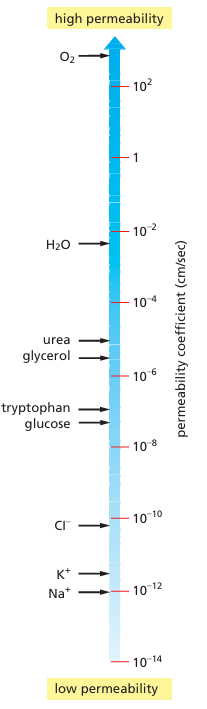
\includegraphics[height = 8cm]{2}
	}
	% Second subfigure
	\subfigure[Relative permeability]{
		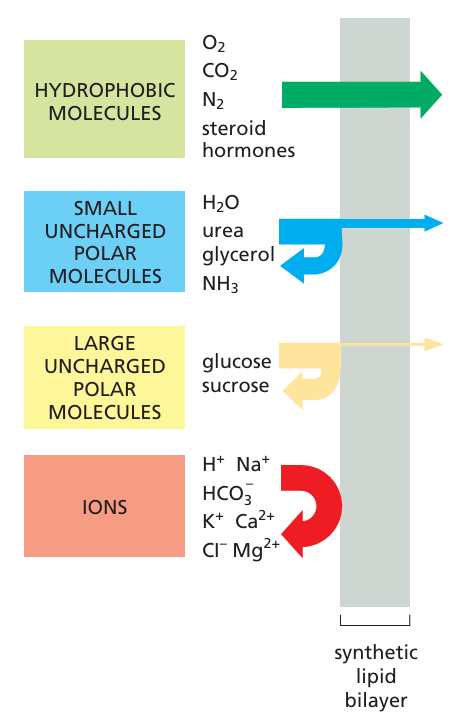
\includegraphics[height = 8cm]{3}
		\label{reactivity}
	}
	\caption{Permeability of the cellular membrane}
\end{figure}
Nevertheless these rates are pretty shit. Therefore in order to benefit from this barrier cells have had to evolve ways of transferring specific water-soluble molecules and ions across their membranes in order to ingest essential nutrients, excrete metabolic waste products, and regulate intracellular ion concentrations. Cells use specialized membrane transport proteins to accomplish this goal. 
\begin{RemarkWithTitel}{Transporters vs Channels}
	There are 2 main classes of \textbf{membrane transport proteins}:  \\
	textbf{Transport Proteins} bind the \textbf{specific solute} to be transported and undergo a series of conformational changes that alternately expose solute-binding sites on one side of the membrane and then on the other to transfer the solute across it.\\
	\textbf{Channels}, by contrast, interact with the solute to be transported much more weakly (no conformational changes). They form continuous pores that extend across the lipid bilayer.\\
	Not surprisingly transport through channels occures at a much faster rate then transport mediated by transporters.
\end{RemarkWithTitel}
\begin{RemarkWithTitel}{Active vs Passiv Transport}
	All channels and many transporters allow solutes to cross the membrane only passively ("downhill"), this is called \textbf{passive transport}. In this case of an uncharged molecule the driving force is the concentration gradient while charged molecules are influenced by the membrane potential (electrochemical gradient). \\
	There also transport "uphill", against the eletrochemical gradient. Such \textbf{active transport} is mediated by transporters whose pumping pumping activity is directional because it is tightly coupled to a source of metabolic energy, such as an ion gradient or ATP hydrolysis. 
\end{RemarkWithTitel} 
\begin{figure}[H]
	\centering
	\subfigure[Active vs Passive Transport]{
		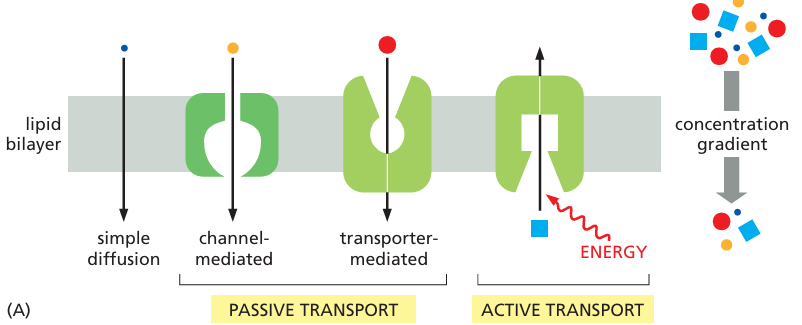
\includegraphics[width = 0.55\textwidth]{5}
	}
	% Second subfigure
	\subfigure[Transporters vs Channels]{
		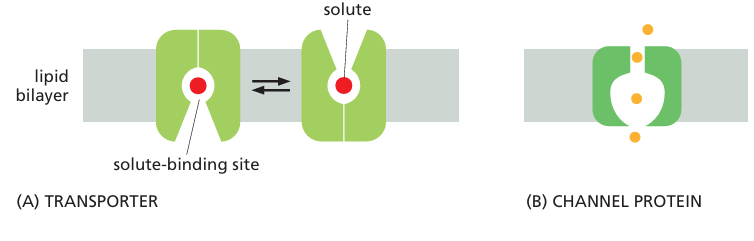
\includegraphics[width = 0.4\textwidth]{1}
		\label{reactivity}
	}
	\caption{Transport Membrane Proteins}
\end{figure}


\subsubsection{Ion concentrations}
The barrier function of the cell membrane allows the cell to maintain concentrations of solutes in its cytosol that differ from those in the extracellular fluid. \textbf{The cell membrane is particularly impermeable to ions.} \\
Note that a cell must contain equal quantities of positive and negative charges (\textbf{neutral}). The cell contains many other anions not listed in table \ref{tableconc} like inorganic phosphate, nucleic acids, etc. 

\begin{DefWithTitle}{Electrochemical gradient}
	The concentration gradient and the electrical potential difference across the membrane combine to form a \textbf{net driving force} the elctrochemical gradient. 
\end{DefWithTitle}
\begin{figure}[H]
	\centering
	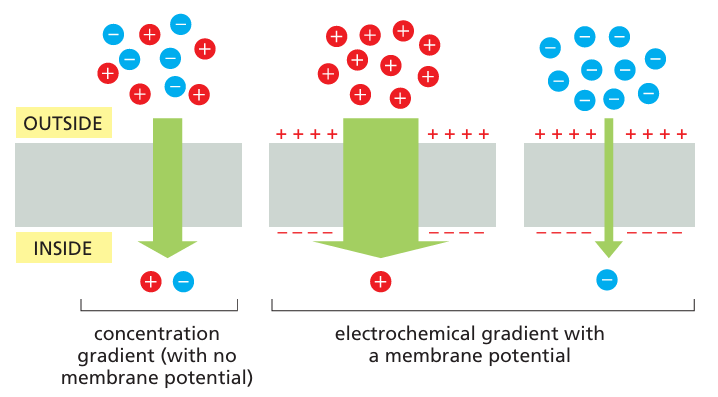
\includegraphics[height = 6cm]{4}
	\caption{The electrochemical gradient of a charged solute (an ion) affects its transport}
\end{figure}
\noindent
The equilibrium potential for ion \(i\) is given by the Nernst equation:
\[
E_i = \frac{RT}{zF} \ln\left(\frac{[ion]_{\text{outside}}}{[ion]_{\text{inside}}}\right)
\]


\begin{table}[h!]
	\centering
	\begin{tabular}{|l|p{3.5cm}|p{3.5cm}|p{3cm}|p{3.5cm}|}
		\hline
		\textbf{Ion} & \textbf{Concentration Inside the Cell (mM)} & \textbf{Concentration Outside the Cell (mM)} & \textbf{Equilibrium Potential (E\textsubscript{i}) (mV)} & \textbf{Direction of Movement} \\ \hline
		Na\textsuperscript{+} & 5--15 & 145 & +60 & \textbf{Inward} (strong chemical and electrical gradients) \\ \hline
		K\textsuperscript{+}  & 140 & 5 & -90 & Outward but opposing forces \textbf{nearly balanced}, near equilibrium \\ \hline
		Ca\textsuperscript{2+} & $10^{-4}$ & 1--2 & +120 & \textbf{Inward} (very strong chemical and electrical gradients) \\ \hline
		Mg\textsuperscript{2+} & 0.5 & 1--2 & -10 to -20 & \textbf{Outward} or near equilibrium (small gradient) \\ \hline
		H\textsuperscript{+} & $7 \times 10^{-5}$ (10\textsuperscript{-7.2} M or pH 7.2) & $4 \times 10^{-5}$ (10\textsuperscript{-7.4} M or pH 7.4) & Varies with pH & Varies (affects pH balance, weak gradient under normal conditions) \\ \hline
		Cl\textsuperscript{-} & 5--15 & 110 & -70 to -80 & Inward but opposing forces \textbf{nearly balanced}, near equilibrium  \\ \hline
	\end{tabular}
	\caption{Ion Concentrations and Equilibrium Potentials}
	\label{tableconc}  % Label added here
\end{table}
Note that the \textbf{resting membrane potential is around -70 mV} = Vm.  Using this one can calculate the driving force for an \textbf{cation }across the membrane (att. for neg charge switch). 
\[
\Delta E_i = E_i - V_m
\]
\begin{itemize}
	\item \( \Delta E_i > 0 \): The ion will move \textbf{inward} (from outside to inside the cell),
	\item \( \Delta E_i < 0 \): The ion will move \textbf{outward} (from inside to outside the cell),
	\item \( \Delta E_i = 0 \): There is no net movement of that ion (the ion is at equilibrium).
\end{itemize}

Note that the movement of only a minute number of inorganic ions across the plasma membrane through ion channels suffices to set up the membrane potential. Thus, we can think of the membrane potential as arising from movements of charge that leave ion concentrations practically unaffected.  

\begin{ExWithTitle}{Acetylcholine-gated cation channels do not discriminatie between Na+, K+ or Ca++. But when they open mostly Na+ enters the cell.}
	There is little net movement of K+ because it is nearly at equilibrium distribution, by contrast Na+  and Ca++ are not at equilibrium distribution. However Ca++ is present in way lower concentration then Na+. Therefore Na+ enters the cell. 
\end{ExWithTitle}



\subsection{Transporters}
Transporters are typically built from bundles of \textbf{10 or more $\alpha$ helices} that span the membrane. \textbf{Solute- and ion-binding sites are located midway through the membrane}, where some helices are broken or distorted and amino acid side chains form ion- and solute-binding sites. \\
In the inward-open and outward-open conformations, these binding sites are accessible by passageways from one side of the membrane but not the other. The switching between the two conformations. The switching between these two (3) states transfers the solute from one side to the other. See fig. \ref{modeltransprot}\\
\\
Moreover Transporters are build from inverted repeats. This leads to the fact that the repeats can move relative to each other. Therefore opening one side leads to the closing of the other. 

\begin{figure}[H]
	\centering
	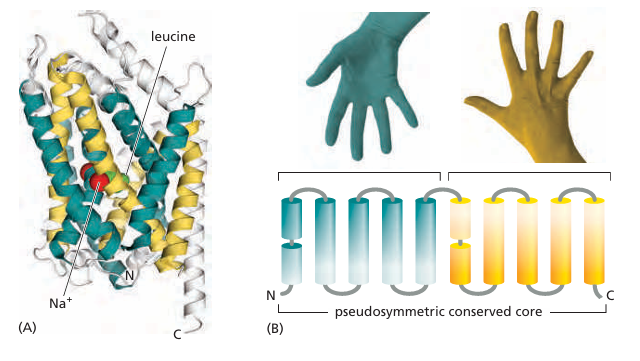
\includegraphics[height = 6cm]{8}
	\caption{Transporters are built from inverted repeats.}
\end{figure}



In many ways \textbf{Transporters behave like enzymes}. Each type of transporter has one ore more \textbf{specific binding sites for its solute}. Moreover, when the transporter is saturated, the rate of transport is maximal (\textbf{Vmax}), is characteristic of a specific carrier. In addition, each transporter has a characteristic affinity for its solute, reflected in the \textbf{Km} of the reaction, which is equal to the concentration of solute when the transport rate is half its maximum value. There can also be an interplay with an inhibitor.  See fig. \ref{kineticsoftransporters}
\begin{figure}[H]
	\centering
	\subfigure[Model for passive transport]{
		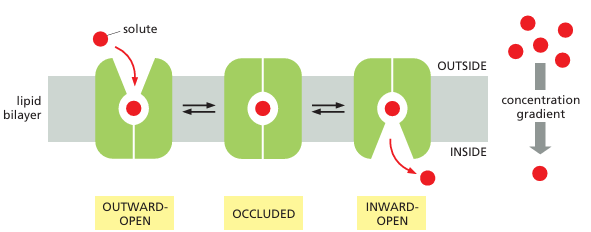
\includegraphics[width = 0.6\textwidth]{10}
		\label{modeltransprot}
	}
	% Second subfigure
	\subfigure[Kinetics of Transporters]{
		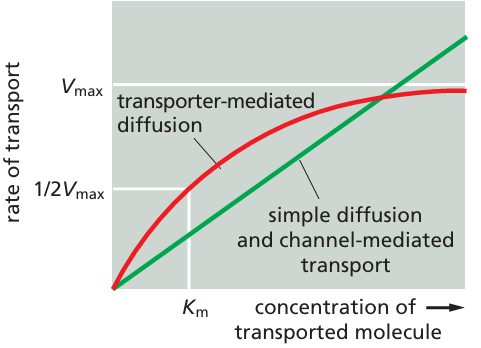
\includegraphics[width = 0.3\textwidth]{6}
		\label{kineticsoftransporters}
	}
	\caption{}
\end{figure}


Apart from passive transport, trasnporters can also engage in active transport. There are strong similarities in structure between transporters that mediate active transport and those that mediate passive transport. This suggests an evolutionary relationship. \\
There are 3 main ways of driving active transport: 
\begin{itemize}
	\item \textbf{Coupled transporters} harness the energy stored in concentration gradients to couple the uphill transport of one solute across the membrane to the downhill transport of another. 
	\item \textbf{ATP-driven pumps} couple uphill transport to the hydrolysis of ATP
	\item Light- or redox-driven pumps, which are known in bacteria, archaea, mitochondria, and chloroplasts, couple uphill transport to an input of energy from light.
\end{itemize}


\begin{figure}[H]
	\centering
	\subfigure[Three ways of driving active transport]{
		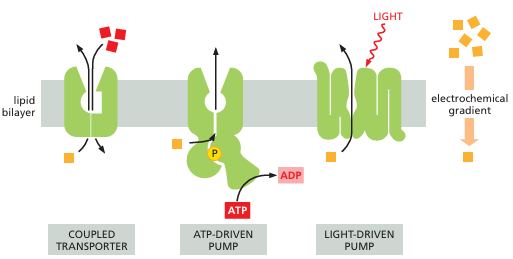
\includegraphics[width = 0.5\textwidth]{7}
	}
	% Second subfigure
	\subfigure[Transporters functioning as uniporters, symporters, and antiporters ]{
		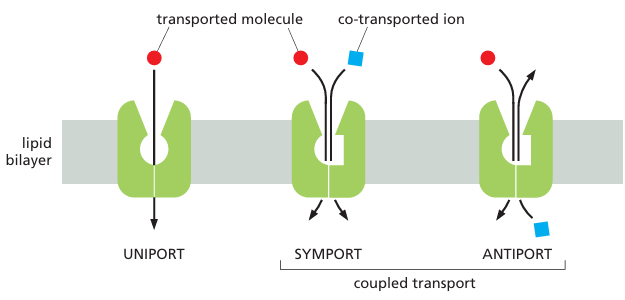
\includegraphics[width = 0.45\textwidth]{9}
		\label{uniporters}
	}
	\caption{}
\end{figure}

\subsubsection{Active Transport driven by Ion-Concentration Gradients}
Some Transporters simply \textbf{passively} mediate the movement of a single solute from one side of the membrane; they are called \textbf{\gls{uniporter}}. See. Fig. \label{uniporters}\\
\\
Others function as \textbf{coupled trnsporters} (type of active transport), in which the transfer of one solute strictly depends on the transport of a second. In some the coupled transport is performed in the same direction (\textbf{\gls{symporter}}), while in others the transport is performed in oposit directions (\textbf{\gls{antiporter}}). See. Fig. \label{uniporters}\\
\\
The tight coupling between the transfer of two solutes allows the coupled transporters to harvest the energy stored in the electrochemical gradient of one solute, typically an inorganic ion, to transport the other. \\
\\
\textbf{Na+ is the usual co-transported ion} because its electrochemical gradient provides a large driving force for the active transport of a second molecule. The Na+ that enters the cell during coupled transport is \textbf{subsequently pumped out by an ATP-driven Na+-K+ pump} in the plasma membrane, which, by maintaining the Na+ gradient, indirectly drives the coupled transport. \\
Such ion-driven transport is called \textbf{\gls{secondaryactivetransport}}, while the ATP-driven pump are said to mediate \textbf{\gls{primaryactivetransport}} 	

\begin{figure}[H]
	\centering
	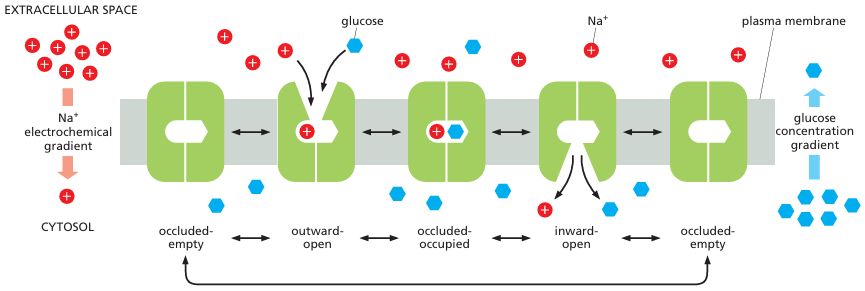
\includegraphics[width = 0.8 \textwidth]{11}
	\caption{Mechanism of glucose transport fueled by a Na+ gradient (\textbf{\gls{SGLT}})}
\end{figure}

\paragraph{Transcellular Transport}
In epithelial cells, such as those that absorb nutrients from the gut, transporters are \textbf{distributed nonuniformly} in the plasma membrane and thereby contribute to the transcellular transport of absorbed solutes. \textbf{Transporters are evolutionary placed where it makes sense for the cell.}\\
\\
Na+-linked symporters (\textbf{SGLT1}) located in the apical (absorptive) domain of the plasma membrane a\textbf{ctively transport nutrients into the cell}, building up substantial concentration gradients.\\
\textbf{Uniporters} in the basal and lateral (basolateral) domains allow the nutrients to leave the cell \textbf{passively down these concentration gradients}. (See fig. \ref{AsymmetrionDistributionofTransporters})

\begin{figure}[H]
	\centering
	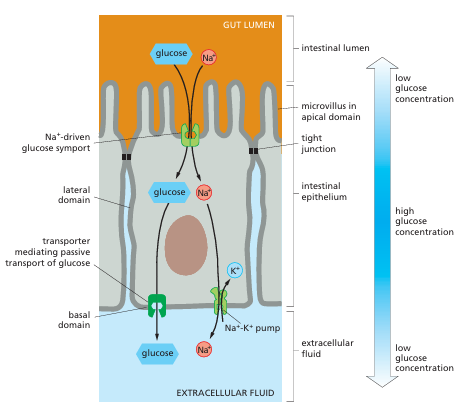
\includegraphics[height = 8cm]{12}
	\caption{An Asymmetric Distribution of Transporters in Epithelial Cells Underlies the Transcellular Transport of Solutes}
	\label{AsymmetrionDistributionofTransporters}
\end{figure}


\subsubsection{Active Transport by ATP-Driven Pumps}
There are 3 classes of ATP driven pumps (also often called \textbf{transport ATPases} because the hydrolyze ATP to ADP). 
\begin{itemize}
	\item \textbf{P-type} pumps are structurally and functionally related \textbf{multipass transmembrane proteins}. They are called “P-type” because \textbf{they phosphorylate themselves} during the pumping cycle. This class includes many of the \textbf{ion pumps} that are responsible for setting up and maintaining gradients of \textbf{Na+, K+, H+, and Ca2+} across cell membranes.
	\item \textbf{ABC transporters} (ATP-Binding Cassette transporters) differ structurally from P-type ATPases and primarily pump \textbf{small molecules} across cell membranes.
	\item \textbf{V-type} pumps are turbine-like protein machines, constructed from \textbf{multiple different subunits}. The V-type proton pump transfers \textbf{H+ into organelles}.
\end{itemize}

\begin{figure}[H]
	\centering
	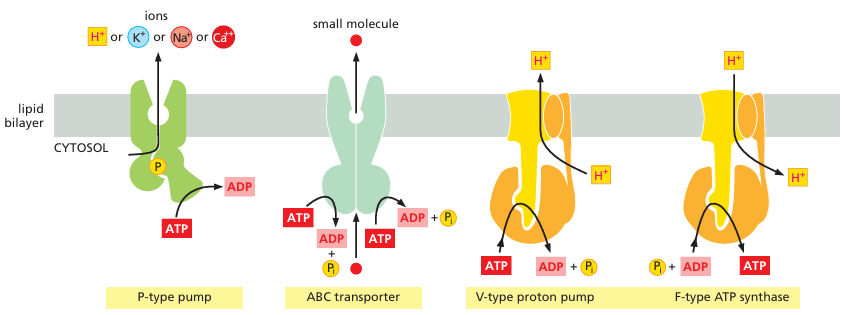
\includegraphics[width = 0.8 \textwidth]{13}
	\caption{Three types of aTP-driven 
		pumps.}
\end{figure}

\paragraph{Na+/K+ pump}
The Na+/K+ ATPase is a \textbf{ATP-driven antiporter P-type ATPase.} It maintains the \textbf{Na+ gradient} important for the transport of ntirens into the cells (\textbf{osmotic balance}). The importance is underlined by the fact that 1/3 of the cells energy is devoted to this pump.\\
\\
Since the Na+-K+ pump drives three positively charged ions out of the cell for every two it pumps in, it is \textbf{electrogenic}: it drives a net electric current across the membrane. This corresponds to about 10 \% of the membrane potential. 

\begin{figure}[H]
	\centering
	\subfigure[Function of the Na+/K+ pump]{
		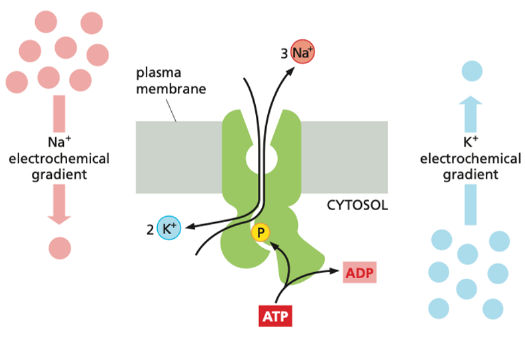
\includegraphics[width = 0.35\textwidth]{15}
	}
	% Second subfigure
	\subfigure[The cycle of the Na+/K+ pump]{
		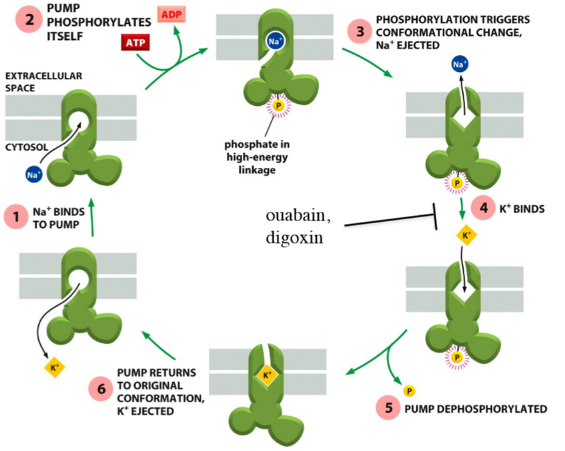
\includegraphics[width = 0.6\textwidth]{14}
		\label{uniporters}
	}
	\caption{Na+/K+ pump}
\end{figure} 

\begin{RemarkWithTitel}{Osmolarity}
	\textbf{\gls{osmolarity}} is a measure of the total concentration of solute particles in a solution. It determines the direction of water movement across membranes: water tends to move from areas of lower to higher osmolarity. In cells, the Na\textsuperscript{+}/K\textsuperscript{+} pump helps regulate osmolarity by exporting more ions than it imports, thereby reducing intracellular solute concentration and helping to prevent excessive water entry. This regulation is essential for maintaining cell volume and structure, keeping the cell \textbf{\gls{isotonic}} rather than \textbf{\gls{hypertonic}} or \textbf{\gls{hypotonic}}.
\end{RemarkWithTitel}

\paragraph{Ca2+ pump}
The Ca2+ pump, or Ca2+ ATPase, in the sarcoplasmic reticulum (SR) membrane of skeletal muscle cells is a well-understood P-type transport ATPase.
\begin{RemarkWithTitel}{\gls{sarcoplasmicreticulum}}
	The SR is a specialized type of endoplasmic reticulum that forms a network of tubular sacs in the muscle cell cytoplasm, and it serves as an intracellular store of Ca2+. 
\end{RemarkWithTitel}
When an action potential depolarizes the muscle cell plasma membrane, Ca2+ is released into the cytosol from the SR through Ca2+-release channels, stimulating the muscle to contract. \\
The Ca2+ pump, which accounts for about 90 \% of the membrane protein of the SR, moves Ca2+ from the cytosol back into the SR. The endoplasmic reticulum of nonmuscle cells contains a similar Ca2+ pump, but in smaller quantities.
\begin{figure}[H]
	\centering
	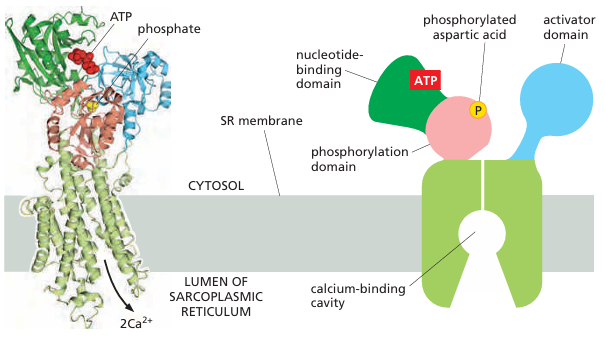
\includegraphics[width = 0.6 \textwidth]{16}
	\caption{The structure of the sarcoplasmic reticulum Ca2+ pump.}
\end{figure}
Ca2+ binding triggers a series of conformational changes that close the passageway to the cytosol and activate a phosphotransfer reaction in which the terminal phosphate of the \textbf{ATP is transferred to an aspartate that is highly con served among all P-type ATPases}. The ADP then dissociates and is replaced with a fresh ATP, causing another conformational change that opens a passageway to the SR lumen through which the two Ca2+ ions exit. They are replaced by two H+ ions and a water molecule that stabilize the empty Ca2+-binding sites and close the passageway to the SR lumen. Hydrolysis of the labile phosphoryl-aspartate bond returns the pump to the initial conformation, and the cycle starts again. See fig. \ref{sarcoplasmic_reticulum_pump}
\begin{figure}[H]
	\centering
	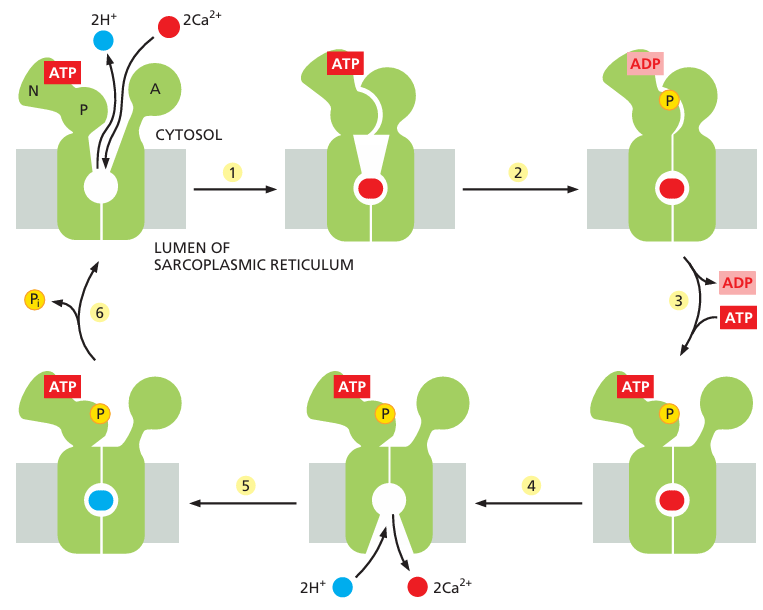
\includegraphics[width = 0.7 \textwidth]{17}
	\caption{The pumping cycle of the sarcoplasmic reticulum Ca2+ pump. }
	\label{sarcoplasmic_reticulum_pump}
\end{figure}

\paragraph{ABC-Transporters}
They are a large fammily of membrane transport proteins (ex: 5\% of E.coli genome). There exist 48 proteins in humans. \\
ABC transporters contains \textbf{two highly conserved ATPase domains}, or ATP-Binding “Cassettes,” on the cytosolic side of the membrane. ATP binding brings together the two ATPase domains (dimerization), and ATP hydrolysis leads to their dissociation. \\
They transport a high variety of substrates: sugar, amino acids, drugs, antibiotics, toxins, lipids, peptides, nucleotides and more. 

\begin{figure}[H]
	\centering
	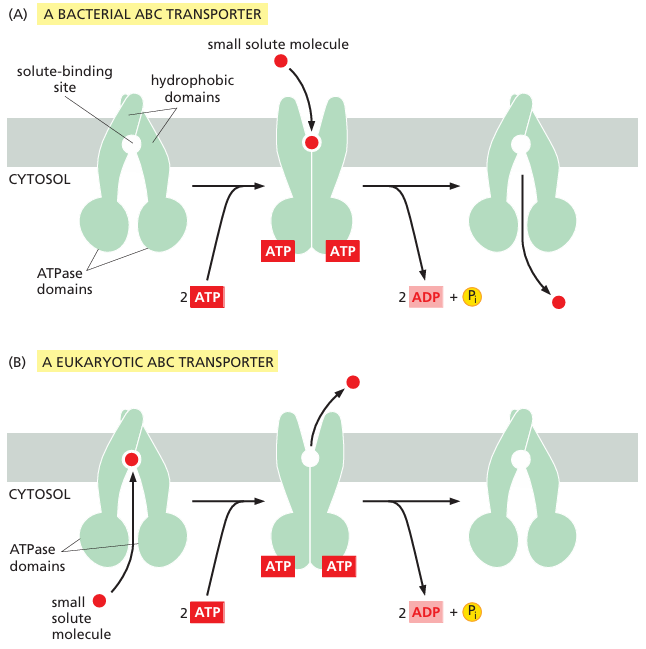
\includegraphics[width = 0.7 \textwidth]{18}
	\caption{Small-molecule transport by typical ABC transporters.}
	\label{ABCtransporter}
\end{figure}
\textit{Note in eukaryotes, most ABC transporters export substances.}

\begin{RemarkWithTitel}{\gls{multidrugresistance}}
	A phenomenon where cells become resistant to a wide range of structurally unrelated drugs, often due to the activity of \textbf{MDR proteins} (ABC transporters) that actively export toxic substances and therapeutic drugs out of the cell, reducing their intracellular concentrations and effectiveness.\\
	Note these MDR proteins can also promote resistance to chemotherapies. 
\end{RemarkWithTitel}

\subsection{Channels} 
Unlike transporters, channels form pores across membranes. One class of channel proteins found in virtually all animals forms \textbf{gap junctions} between adjacent cells.\\
As discussed earlier, however, channels cannot be coupled to an energy source to perform active transport, so the transport they mediate is always passive (downhill).

\subsubsection{Aquaporins}
Aquaporins solve a problem that is opposite to that facing ion channels. To avoid disrupting ion gradients across membranes, they have to allow the \textbf{rapid passage of water molecules} while completely blocking the passage of ions. The three-dimensional structure of an aquaporin reveals how it achieves this remarkable selectivity. \\
\\
The channels have a narrow pore that allows water molecules to traverse the membrane in single file, following the path of carbonyl oxygens that line one side of the pore. \\
Hydrophobic amino acids line the other side of the pore. The pore is too narrow for any hydrated ion to enter, and \textbf{the energy cost of dehydrating an ion would be enormou}s because the hydrophobic wall of the pore cannot interact with a dehydrated ion to compensate for the loss of water. Therefore K+ and other ions can not transfer through aquaporins. \\
\\
Moreover these channels are also impermeable to H+. Because aquaporins contain \textbf{two strategically placed asparagines}, which bind to the oxygen atom of the central water molecule in the line of water molecules traversing the pore, imposing a bipolarity on the entire column of water molecules. This makes it impossible for the “making and breaking” sequence of hydrogen bonds to get past the central asparagine-bonded water molecule, because both valences of this central oxygen are unavailable. 

\begin{figure}[H]
	\centering
	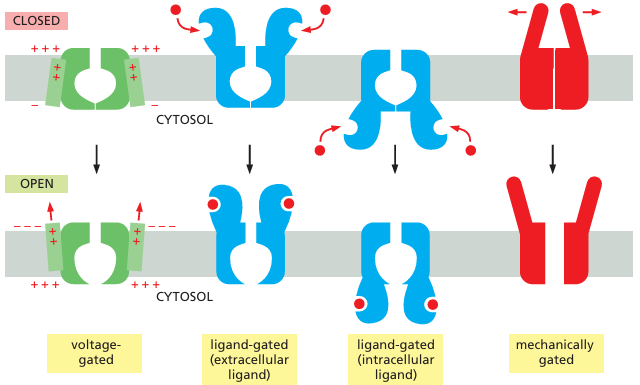
\includegraphics[width = 0.7 \textwidth]{20}
	\caption{The structure of aquaporins}
	\label{aquaporins}
\end{figure}

\begin{RemarkWithTitel}{The response to dehydration}
	\textbf{\gls{vasopressin}} is a peptide hormone released by the posterior pituitary in response to dehydration or increased plasma osmolarity. It promotes water reabsorption in the kidneys by stimulating the insertion of aquaporin-2 channels in the collecting ducts, thereby reducing urine output and conserving body water
\end{RemarkWithTitel}

\subsubsection{Ion channels}
Two important properties distinguish ion channels from aqueous pores.
\begin{itemize}
	\item  First, they show \textbf{ion selectivity}, permitting some inorganic ions to pass, but not others. The permeating ions have to shed most or all of their associated water molecules to pass, often \textbf{in single file}, through the narrowest part of the channel, which is called the \textbf{selectivity filter}; this limits their rate. 
	of passage
	
	\item Second, ion channels are not continuously open. Instead, they are \textbf{gated}, which allows them to open briefly and then close again. In most cases, the gate opens in response 
	to a specific stimulus. See fig. \ref{gatingchannels}
\end{itemize} 

\begin{figure}[H]
	\centering
	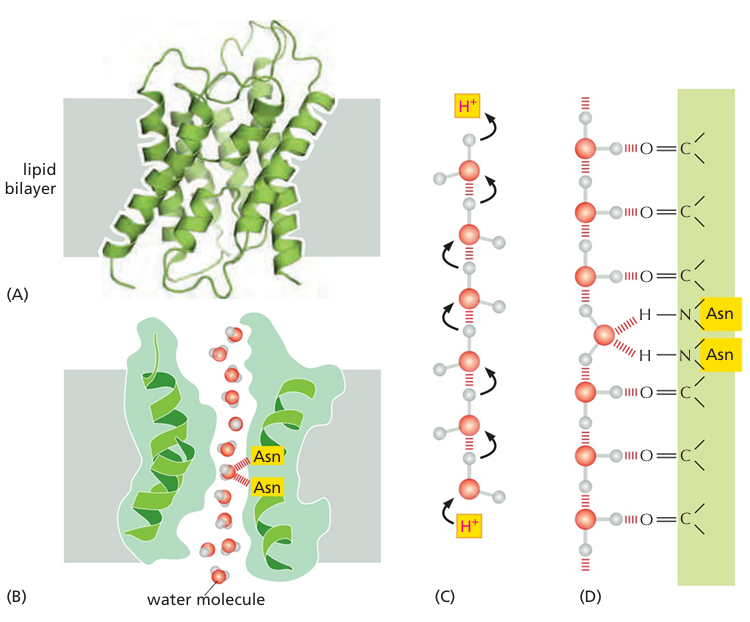
\includegraphics[width = 0.7 \textwidth]{19}
	\caption{The gating of ion channels}
	\label{gatingchannels}
\end{figure}
Moreover, protein \textbf{phosphorylation} and dephosphorylation regulates the activity of many ion channels; this type of channel regulation is discussed, together with nucleotide-gated ion channels. \\
\\
In general, \textbf{gating involves movement of the helices} in the membrane so that they either obstruct or open the path for ion movement. Depending on the particular type of channel, helices tilt, rotate, or bend during gating. \\
\\
Ligand-gated \textbf{channels open and close periodically}. The probability to switch from the closed to the open state depends largely on the concentration of the ligand. But they will always close spontaneously. The simplest way is that the lignad just unbinds. But there are also channels that enter desensitized state while their still bound to the ligand, preventing overfirering.\\
Moreover note that channels always completely open or closed, there is nothin gin between. 
\begin{figure}[H]
	\centering
	\subfigure[ligand-gated]{
		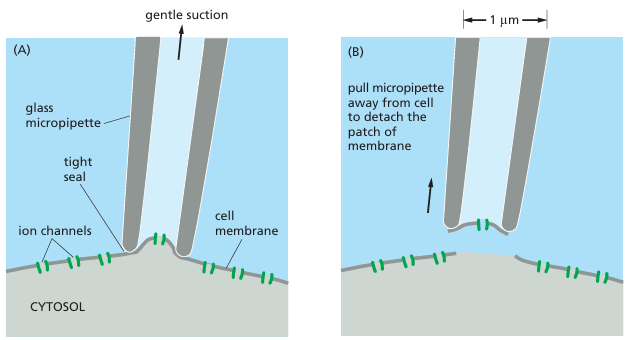
\includegraphics[height = 5cm]{23}
	}
	% Second subfigure
	\subfigure["All or Nothing" fashion]{
		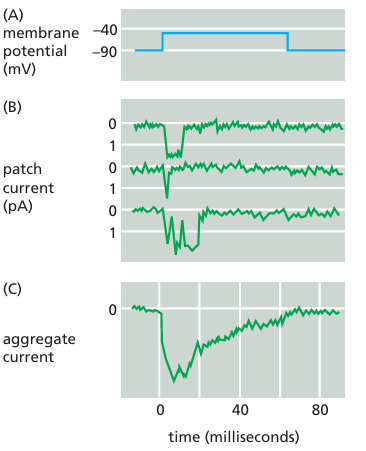
\includegraphics[height = 5cm]{24}
	}
	\caption{}
\end{figure} 


\paragraph{K+ (leak) channels}
Ion channels that are permeable mainly to K+ are found in the plasma membrane of almost all cells. An important subset of K+ channels opens even in an unstimulated or “resting” cell, and hence these are called K+ leak channels.\\
\\
K+ leak channels conduct K+ 10,000-fold faster than Na+, yet the two ions are both featureless spheres and have similar diameters (0.133 nm and 0.095 nm, respectively).

The polypeptide chain that connects the two transmembrane helices forms a short $\alpha$ helix (the pore helix) and a crucial loop that protrudes into the wide section of the cone to form the \textbf{selectivity filter}. In this filter functions thanks to the \textbf{coordination between carbonyl oxygens and the dehydrated K+}. \\
Moreover, they channel attracts cation by negative charged amino acids. See fig. \ref{structureK+}
\begin{figure}[H]
	\centering
	\subfigure[The structure of a bacterial K+ channel.]{
		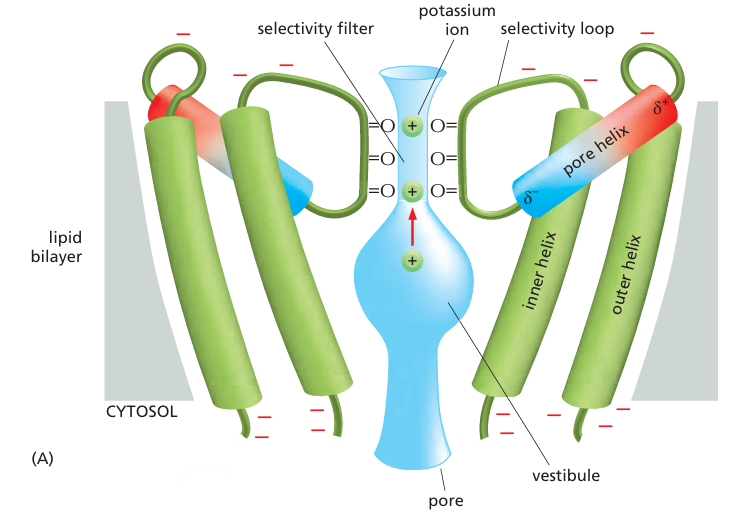
\includegraphics[width = 0.5\textwidth]{21}
	}
	% Second subfigure
	\subfigure[K+ specificity of the selectivity filter in a K+ channel. ]{
		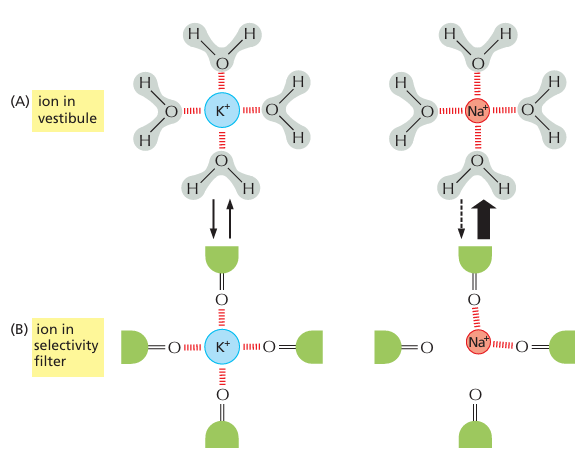
\includegraphics[width = 0.45\textwidth]{22}
	}
	\caption{K+ channel}
	\label{structureK+}
\end{figure} 
Many K+ channels are \textbf{voltage gated} and essential for electrical signaling. 
\begin{RemarkWithTitel}{Electrical signaling}
	At rest, a neuron keeps more K+ inside and more Na+ outside, creating an electrical difference across the membrane. When a signal arrives (action potential starts), voltage-gated Na+ channels open, and Na+ rushes in depolarizing the membrane, making the inside more positive (rising phase of the signal). Shortly after, K+ channels open, and K+ flows out, repolarizing the cell (back to its resting state). When the action potential reaches the end of the neuron, Ca2+ channels open during depolarization, and Ca2+ enters, triggering processes like neurotransmitter release.
\end{RemarkWithTitel}

\paragraph{Patch-clamp}

\gls{patchclamp} is a technique to record ionic current flow through individual channels while membrane potential is clamped. Because of the extremely tight seal between the micropipette and the membrane, current only enter or leave the micropipette by passing through the ion channel in the patch.  \\
\\
This enables to determine which molecules activate the channel on an which side.  
\begin{figure}[H]
	\centering
	\subfigure[The technique of patch-clamp recording]{
		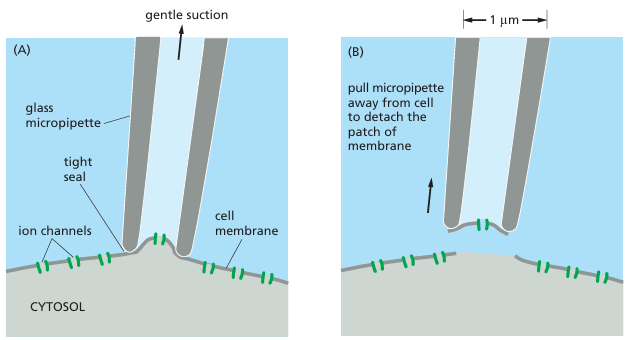
\includegraphics[width = 0.6\textwidth]{23}
	}
	% Second subfigure
	\subfigure[Patch-clamp measurements for a single voltage gated Na+ channel.]{
		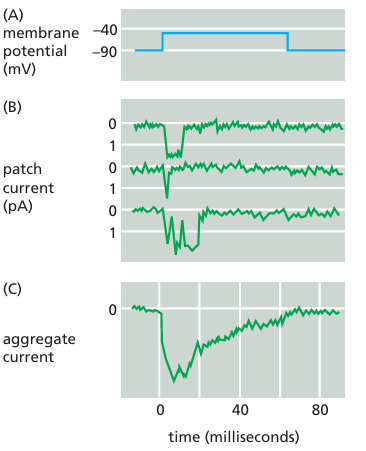
\includegraphics[width = 0.3\textwidth]{24}
	}
	\caption{Patch-clamp}
	\label{patch-clamp}
\end{figure} 
Note that the aggregate current (the sum of multiple experiments) reflects the probability that any individual channel will be in the open state. 

\end{document}